%%%%%%%%%%%%%%%%%%%%%%%%%%%%%%%%%%%%%%%%%
% Proceedings of the National Academy of Sciences (PNAS)
% LaTeX Template
% Version 1.0 (19/5/13)
%
% This template has been downloaded from:
% http://www.LaTeXTemplates.com
%
% Original author:
% The PNAStwo class was created and is owned by PNAS:
% http://www.pnas.org/site/authors/LaTex.xhtml
% This template has been modified from the blank PNAS template to include
% examples of how to insert content and drastically change commenting. The
% structural integrity is maintained as in the original blank template.
%
% Original header:
%% PNAStmpl.tex
%% Template file to use for PNAS articles prepared in LaTeX
%% Version: Apr 14, 2008
%
%%%%%%%%%%%%%%%%%%%%%%%%%%%%%%%%%%%%%%%%%

%----------------------------------------------------------------------------------------
% PACKAGES AND OTHER DOCUMENT CONFIGURATIONS
%----------------------------------------------------------------------------------------

%------------------------------------------------
% BASIC CLASS FILE
%------------------------------------------------

%% PNAStwo for two column articles is called by default.
%% Uncomment PNASone for single column articles. One column class
%% and style files are available upon request from pnas@nas.edu.

\documentclass[a4paper]{article}
%\documentclass{pnastwo}

%------------------------------------------------
% POSITION OF TEXT
%------------------------------------------------

%% Changing position of text on physical page:
%% Since not all printers position
%% the printed page in the same place on the physical page,
%% you can change the position yourself here, if you need to:

% \advance\voffset -.5in % Minus dimension will raise the printed page on the 
%  physical page; positive dimension will lower it.

%% You may set the dimension to the size that you need.

%------------------------------------------------
% GRAPHICS STYLE FILE
%------------------------------------------------

%% Requires graphics style file (graphicx.sty), used for inserting
%% .eps/image files into LaTeX articles.
%% Note that inclusion of .eps files is for your reference only;
%% when submitting to PNAS please submit figures separately.

%% Type into the square brackets the name of the driver program 
%% that you are using. If you don't know, try dvips, which is the
%% most common PC driver, or textures for the Mac. These are the options:

% [dvips], [xdvi], [dvipdf], [dvipdfm], [dvipdfmx], [pdftex], [dvipsone],
% [dviwindo], [emtex], [dviwin], [pctexps], [pctexwin], [pctexhp], [pctex32],
% [truetex], [tcidvi], [vtex], [oztex], [textures], [xetex]

\usepackage{graphicx}
\usepackage{algorithmic}
\usepackage{algorithm2e}


%------------------------------------------------
% ADDITIONAL OPTIONAL STYLE FILES
%------------------------------------------------

%% The AMS math files are commonly used to gain access to useful features
%% like extended math fonts and math commands.

\usepackage{amssymb,amsfonts,amsmath}

%------------------------------------------------
% OPTIONAL MACRO FILES
%------------------------------------------------

%% Insert self-defined macros here.
%% \newcommand definitions are recommended; \def definitions are supported

%\newcommand{\mfrac}[2]{\frac{\displaystyle #1}{\displaystyle #2}}
%\def\s{\sigma}


\begin{document}

%----------------------------------------------------------------------------------------
%  TITLE AND AUTHORS
%----------------------------------------------------------------------------------------

\title{Report on Machine Learning Lab, Ex 4} % For titles, only capitalize the first letter


\author{Mostafa Mohamed, Omar Kassem}%\affil{1}{Alberts-Ludwig Universt\"at Freiburg}}
%James Smith\affil{2}{University of Oregon}
%\and
%Jane Smith\affil{1}{}}

%\contributor{Submitted to Proceedings of the National Academy of Sciences of the United States of America}

%----------------------------------------------------------------------------------------

\maketitle % The \maketitle command is necessary to build the title page

%\begin{article}

%----------------------------------------------------------------------------------------
%  ABSTRACT, KEYWORDS AND ABBREVIATIONS
%----------------------------------------------------------------------------------------

%\begin{abstract}
%Abstract
%\end{abstract}

\section{Introduction}
This is a report about the deep learning lab, exercise 4. The general task of this assignment was to use Tensorflow to implement a CNN to train it on solving a search problem and enhancing our results using QLearning. As well as trying different configurations and architectures of the neural networks.

\section{Search problem}
The given problem was find a target position in a given maze. and we need to solve it using an approximation of Q-Learning using neural networks.

\section{Architecture}
\begin{itemize}
\item Network: We used a tensorflow for our neural network, we used a network of 7 hidden layers (combination of convolutions, pooling and dense layers), and sometimes we remove the pooling layers (so only 3 remaining hidden layers)
\item We used an epsilon (for choosing random actions) to be $0.8$ and drops down to $0.05$ after 10,000 iterations.
\end{itemize}

\section{Results}
We tried different configurations for the running.
\begin{itemize}
\item {\bf CNN with pooling,$discount=0.99$}: When we first introduced pooling the average loss instantaneously decreased by a factor of 100, the average loss was around $10^4 - 2 \cdot 10^4$ until 50,000 iterations, but we decided to try different discount value
\item {\bf CNN with pooling, $discount = 0.5$}: The values we tried here had a beginning average loss of $3000$ and it decreased gradually until it reached an average of $300$ in 200,000 iterations.
\item {\bf CNN without pooling, $discount=0.5$}: After setting a lower standard deviation for the weights $10^{-4}$ instead of $0.1$, the loss dropped down to $1.5$ which shows a huge significance, reaching $0.01$ after 30,000 iterations, and consistently remaining less than $0.01$ after 50,000 iterations
\end{itemize}


%----------------------------------------------------------------------------------------
%  FIGURES AND TABLES
%----------------------------------------------------------------------------------------

%% Adding Figure and Table References
%% Be sure to add figures and tables after \end{article}
%% and before \end{document}

%% For figures, put the caption below the illustration.
%%
%% \begin{figure}
%% \caption{Almost Sharp Front}\label{afoto}
%% \end{figure}
\iffalse
\begin{figure}[h]
\centerline{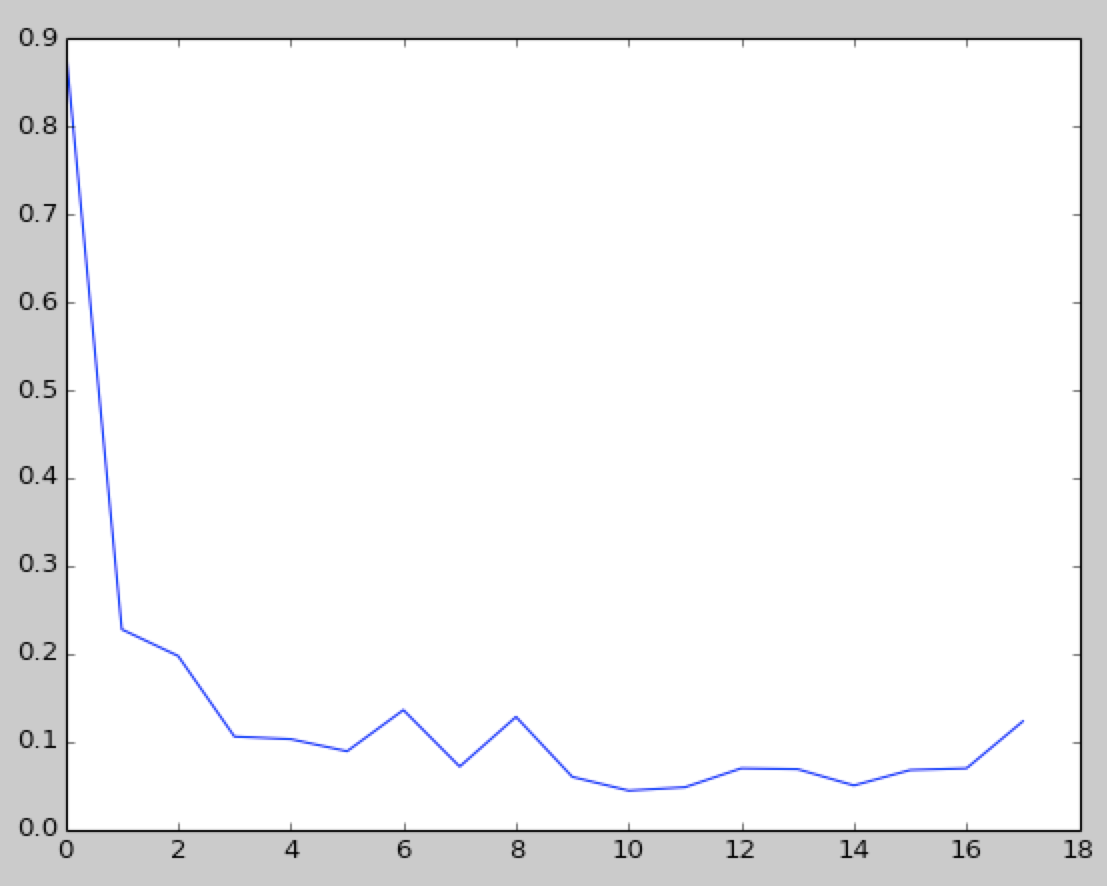
\includegraphics[width=0.4\linewidth]{2L3C.png}}
\caption{2 Layers, 3 Channels, Accuracy: 89\%}\label{placeholder}
\end{figure}

\begin{figure}[h]
\centerline{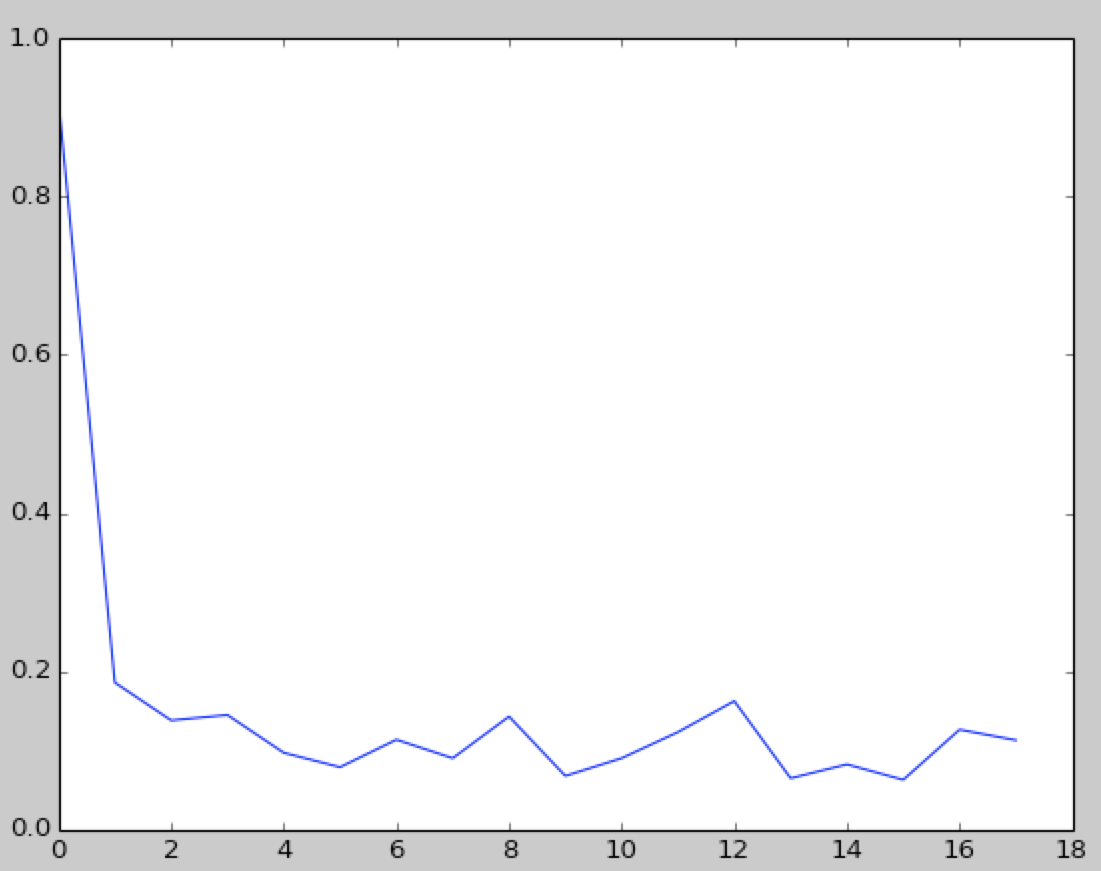
\includegraphics[width=0.4\linewidth]{2L4C.png}}
\caption{2 Layers, 4 Channels, Accuracy: 91\%}\label{placeholder}
\end{figure}

\begin{figure}[h]
\centerline{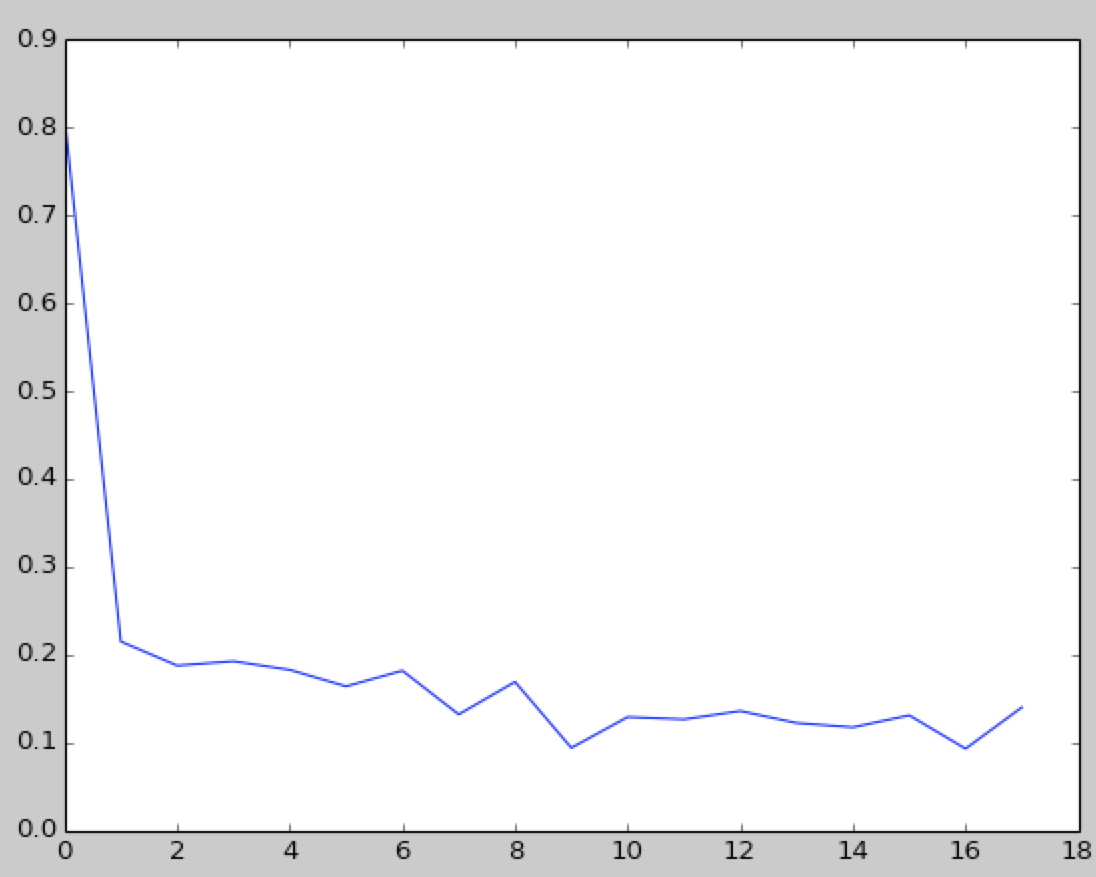
\includegraphics[width=0.4\linewidth]{3L3C.png}}
\caption{3 Layers, 3 Channels, Accuracy: 92\%}\label{placeholder}
\end{figure}

\begin{figure}[h]
\centerline{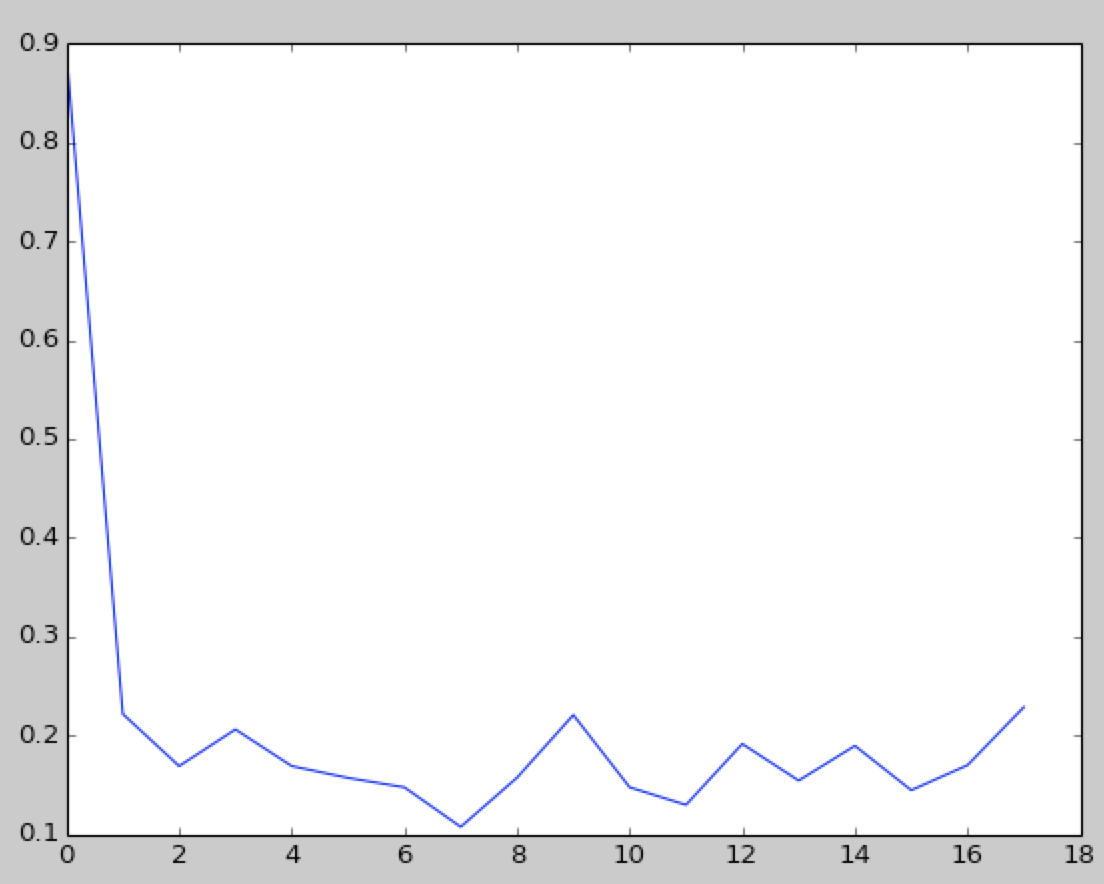
\includegraphics[width=0.4\linewidth]{3L4C.png}}
\caption{3 Layers, 4 Channels, 87\%}\label{placeholder}
\end{figure}
\fi
%% For Tables, put caption above table
%%
%% Table caption should start with a capital letter, continue with lower case
%% and not have a period at the end
%% Using @{\vrule height ?? depth ?? width0pt} in the tabular preamble will
%% keep that much space between every line in the table.

%% \begin{table}
%% \caption{Repeat length of longer allele by age of onset class}
%% \begin{tabular}{@{\vrule height 10.5pt depth4pt  width0pt}lrcccc}
%% table text
%% \end{tabular}
%% \end{table}

%% For two column figures and tables, use the following:

%% \begin{figure*}
%% \caption{Almost Sharp Front}\label{afoto}
%% \end{figure*}

%% \begin{table*}
%% \caption{Repeat length of longer allele by age of onset class}
%% \begin{tabular}{ccc}
%% table text
%% \end{tabular}
%% \end{table*}

%----------------------------------------------------------------------------------------

\end{document}
